\subsubsection{Numero di click}

\begin{longtabu} to \textwidth {| X[0.2,c m] | X[0.1,c m]| X[0.1,c m]| }
    \hline
    \rowcolor{header}
    \textbf{Task} &
    \textbf{Numero di click} &
    \textbf{Esito}\\
    \hline
    caricamento dati da csv & 2 & ottimo \\ 
    \hline
    caricamento dati da server & 3 & ottimo \\
    \hline
    visualizzare i dati & 3 + numero di features & sufficiente \\
    \hline 
    \end{longtabu}


\subsubsection{Site depth}
    L'applicazione web utilizza React e quindi fa in modo che la profondità del sito sia sempre pari ad 1, in quanto tutte le visualizzazioni vengono mostrate quando selezionate e calcolate sulla stessa pagina una alla volta

    
\subsubsection{Response Time}
    Il response time è stato calcolato su file csv di 150 record e i risultati in ms sono i seguenti:

    \begin{figure}[H]
        \centering
        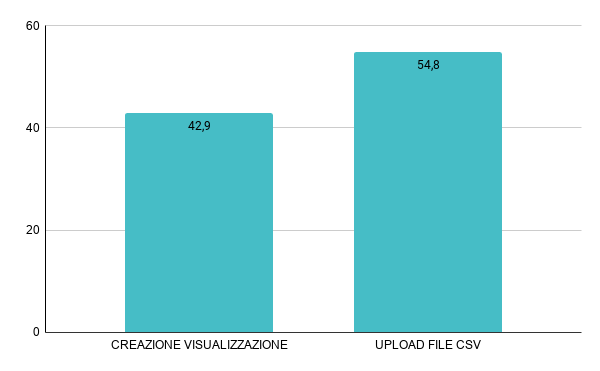
\includegraphics[width=10 cm]{source/sections/images/response-time.png}
        \caption{Grafico del response time}
    \end{figure}
    
\subsubsection{Complessità Ciclomatica}
    Nella seguente tabell e grafico si può vedere i valori della complessità cicolmatica divisi per valori:

        Come si può notare dal segeuente graico il numero di funzioni al di sotto della soglia per considerarsi ottime è pari al 99\%



    \begin{figure}[H]
        \centering
        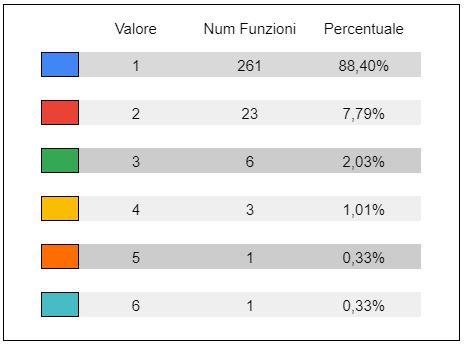
\includegraphics[width=10 cm]{source/sections/images/tabella_CC.JPG}
        \caption{Grafico della percentuale dei test}
    \end{figure}

    \begin{figure}[H]
        \centering
        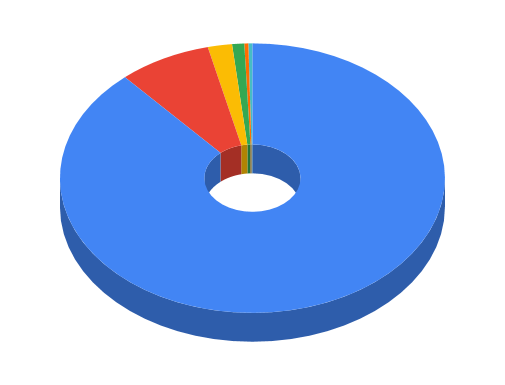
\includegraphics[width=10 cm]{source/sections/images/CC.png}
        \caption{Grafico della percentuale dei test}
    \end{figure}

    \subsubsection{Facilità di comprensione}

        \begin{figure}[H]
            \centering
            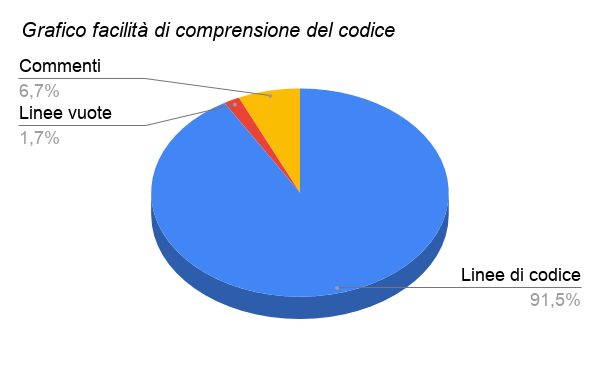
\includegraphics[width=10 cm]{source/sections/images/facilitaDelCodice.png}
            \caption{Grafico della facilità di comprensione}
        \end{figure}

    In seguito i grafici che mostrano l'andamento del numero di righe riguradnati, nel primo grafico il codice, e nel secondo
    le righe di commento e righe vuote

    \begin{figure}[H]
        \centering
        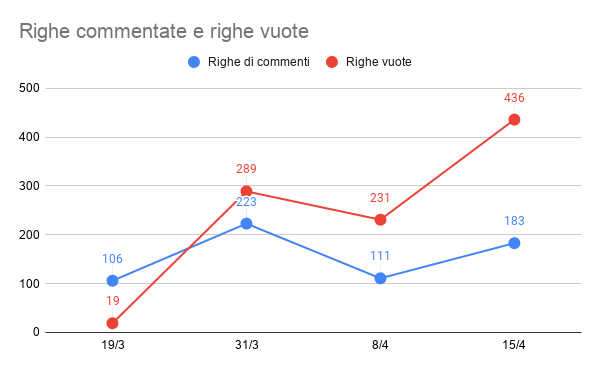
\includegraphics[width=10 cm]{source/sections/images/Valori-delle-righe.png}
        \caption{Grafico del numero di righe dei commenti e righe vuote}
    \end{figure}

    \begin{figure}[H]
        \centering
        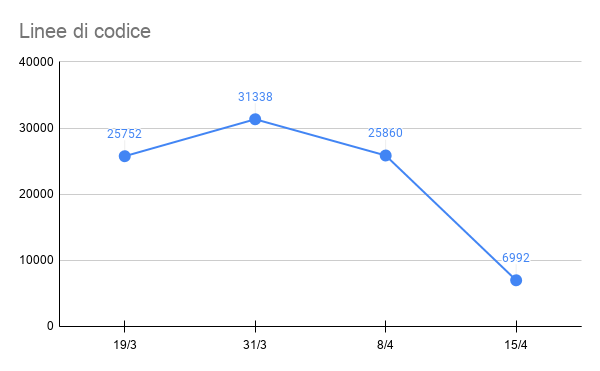
\includegraphics[width=10 cm]{source/sections/images/numCodice.png}
        \caption{Grafico del numero di righe di codice}
    \end{figure}

    \begin{figure}[H]
        \centering
        \includegraphics[width=10 cm]{source/sections/images/facilita_comprensione.png}
        \caption{Grafico della facilità di comprensione}
    \end{figure}

    I forti cambiamenti nell'andamento delle funzioni sono dati da un aggiornamento del progetto fatto in data
    9 Aprile, nel quale si è implementato un comando yarn che si preoccpa di creare la maggiorparte del
    codice CSS, che ha fatto scendere in modo drastico il numero di righe di codice del progetto effettivo. Maggiori chiarimenti nella sezione conclusiva.

\subsubsection{Stractural FAN-in and FAN-out  [sfin and sfout]}
    E' stato calcolato lo Stractural FAN-in e FAN-out di tutti i 44 file del progetto. I risultati sono esposti nella seguente tabella:

    \begin{longtabu} to \textwidth {| X[0.1,c m] | X[0.1,c m] | X[0.1,c m] | X[0.1,c m] | X[0.1,c m] |}
        \hline
        \rowcolor{header}
        \textbf{Esito} &
        \textbf{IN} &
        \textbf{percentiale sul totale} &
        \textbf{OUT} &
        \textbf{percentuale sul totale} \\
        \hline
        Ottimo & 11 & 25\% & 5 & 11,36\% \\ 
        \hline
        Sufficiente & 26 & 59,09\% & 32 & 72,72\% \\ 
        \hline
        Insufficiente & 7 & 15,90\% & 7 & 15,90\% \\ 
        \hline

        \end{longtabu}

        \begin{figure}[H]
            \centering
            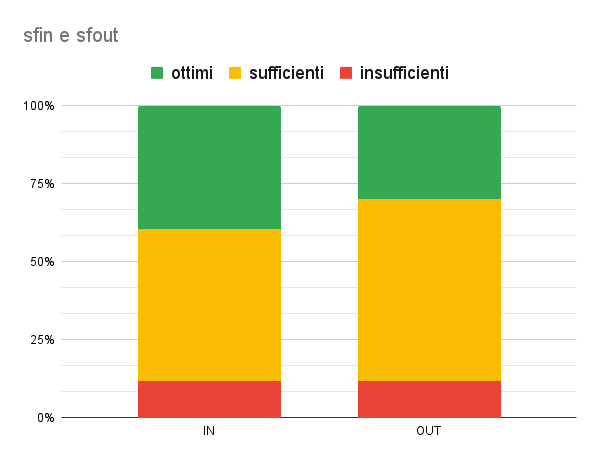
\includegraphics[width=13 cm]{source/sections/images/SfinSfout.png}
            \caption{Grafico delo stractural FAN-in e FAN-out}
        \end{figure}